% ===========================================================================
% SECTION 3 — DATASET GENERATION
% Target: 400-500 words
% ===========================================================================

\section{Dataset Generation}
\label{sec:dataset_generation}

\subsection{Simulation Protocol}
\label{subsec:simulation_protocol}

Training data for the machine learning surrogates is generated by
open-loop simulation of the two-state plant model
(Section~\ref{subsec:two_state_model}) under Region~II/III torque
switching (Section~\ref{subsec:torque_switching}). A total of $80$
trajectories of $300$ time steps each are simulated at $\Delta t =
\SI{0.1}{s}$, giving $80 \times 300 = 24{,}000$ samples. Each trajectory
uses a distinct mean wind speed $V_{\text{mean}}$, superimposed with a
turbulent Kaimal component (Section~\ref{subsec:wind_model}), and a
distinct pitch operating point $\beta_{\text{op}}$; across the 80
trajectories $V_{\text{mean}}$ spans the above-rated envelope up to the
cut-out region (e.g.\ $V_{\text{mean}} = \SI{14.3}{m/s}$ with
$\beta_{\text{op}} = 5.8\deg$ up to $V_{\text{mean}} = \SI{23.9}{m/s}$ with
$\beta_{\text{op}} = 25.0\deg$). The pitch input is excited with a
pseudo-random binary sequence (PRBS), $f_{\text{switch}} = \SI{0.5}{Hz}$,
step amplitude $\delta \in [1,3]\deg$, so that the surrogate training set
captures the local input-output sensitivity needed for one-step-ahead
prediction. Rotor speed initialization is deliberately widened down into
Region~II ($\omegar$ as low as $\approx\SI{8}{rpm}$, consistent with the
torque-switching-constrained range identified in
Section~\ref{subsec:torque_switching}) so that the resulting surrogates
generalize across the Region~II/III boundary rather than only in
above-rated operation.

\subsection{Dataset Structure}
\label{subsec:dataset_structure}

Each sample consists of a feature vector
$X = [\omegar,\ \beta,\ V,\ u_{\text{cmd}}]$ and a one-step-ahead target
$Y = [\omegar^{+},\ \beta^{+}]$, where $u_{\text{cmd}} = \betacmd$ is the
pitch demand applied at the current step and the superscript $+$ denotes
the state at $t+\Delta t$. The $24{,}000$ samples are split at the
\emph{trajectory} level, not the sample level, into $56$ training, $12$
validation, and $12$ test trajectories ($70\%/15\%/15\%$, random seed
$42$), giving $16{,}800$ training, $3{,}600$ validation, and $3{,}600$ test
samples. Splitting by trajectory rather than by individual sample preserves
temporal continuity within each subset and prevents information leakage
across adjacent time steps of the same trajectory, which is essential for a
fair evaluation of the sequence-based surrogates (LSTM, TCN,
Section~\ref{sec:ml_surrogates}) that would otherwise see near-duplicate
windows straddling the train/test boundary. Feature and target
normalization ($z$-score) is computed exclusively on the training split and
applied identically to validation and test data, avoiding any leakage of
validation/test statistics into the training pipeline.

\subsection{Feature Statistics}
\label{subsec:feature_statistics}

Table~\ref{tab:feature_stats} summarizes the operating envelope covered by
the generated dataset. The rotor speed ranges from $\SI{10.28}{rpm}$ to
$\SI{13.31}{rpm}$ (the upper bound coinciding with the plant's maximum
admissible speed, Section~\ref{subsec:nrel5mw}), the pitch angle spans its
full physical domain $[0,25]\deg$, and the wind speed ranges from
$\SI{7.85}{m/s}$ to the cut-out limit of $\SI{25.0}{m/s}$. The maximum
sampled power coefficient is $\Cp^{\max} = 0.480$, consistent with the
Stage~0 Betz-limit validation (Section~\ref{subsec:two_state_model}) and
confirming that no sample in the dataset violates aerodynamic feasibility.
A full dataset validation pass additionally confirmed the absence of
NaN/Inf values, physically consistent one-step increments
($\Delta\omegar$: mean $\SI{0.0030}{rpm}$, std $\SI{0.0217}{rpm}$, max
$\SI{0.1273}{rpm}$ per step; $\Delta\beta$: mean $-0.0006\deg$, std
$0.3250\deg$, max $0.8000\deg$ per step, consistent with the pitch rate
limit $\dot\beta_{\max}$), and correctly normalized training features
(zero mean, unit variance).

\begin{table}[H]
	\centering
	\caption{Dataset feature statistics (24{,}000 samples, 80 trajectories).}
	\label{tab:feature_stats}
	\begin{tabular}{lccc}
		\toprule
		Feature & Min & Max & Unit \\
		\midrule
		$\omegar$ & 10.28 & 13.31 & rpm \\
		$\beta$   & 0.00  & 25.00 & deg \\
		$V$       & 7.85  & 25.00 & m/s \\
		$u_{\text{cmd}}$ & 0.00 & 25.00 & deg \\
		$\Cp$ (sample max) & \multicolumn{2}{c}{0.480 (Betz = 0.5926)} & -- \\
		\bottomrule
	\end{tabular}
\end{table}

\begin{figure}[H]
	\centering
	 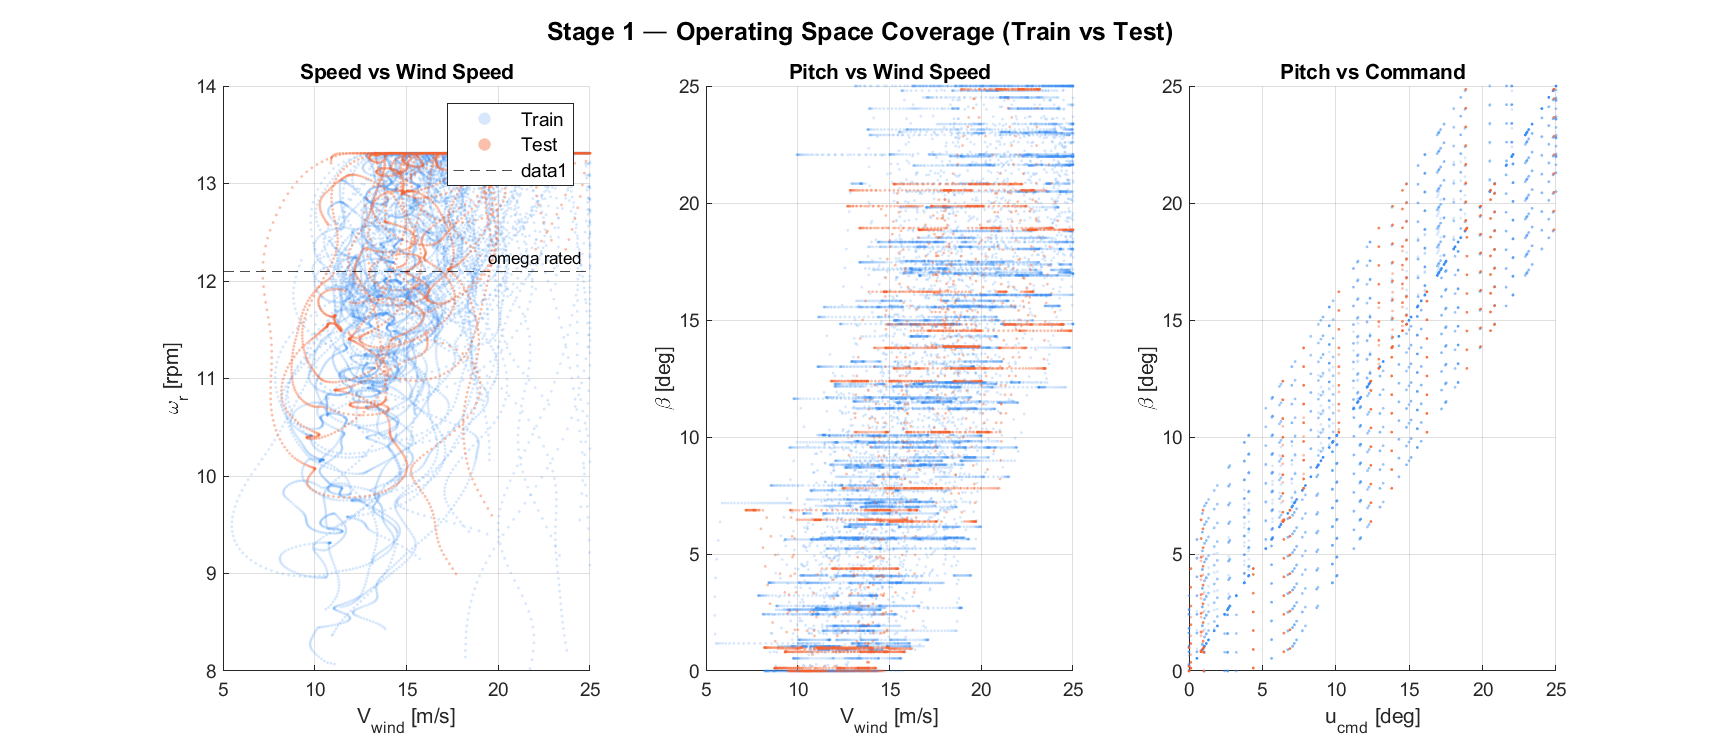
\includegraphics[width=1\textwidth]{figures/Fig1_S1_Coverage.png}
	\caption{Operating-space coverage of the generated dataset: rotor speed
		$\omegar$ versus wind speed $V$, training set (56 trajectories) versus
		test set (12 trajectories).}
	\label{fig:dataset_coverage}
\end{figure}